%% ═══════════════════════════════════════════════════════════════════════════
\section{Technical Supplement}
\label{app:technical}
%% ═══════════════════════════════════════════════════════════════════════════

The body states the model, the experiment and what was measured. This appendix
holds the apparatus behind them: the symbol table, the elicitation and outranking
methods in full, the specification of the forecast layer, and the cost of every
operation. It is written to be consulted rather than read through.


\subsection{Notation}
\label{sec:model_notation}

Table~\ref{tab:notation} fixes every symbol used in this section and the next. Two
conventions are worth stating before the table rather than after it. Subscript $i$ always
indexes a node and subscript $m$ always indexes one of the six KPI blocks, so
$u_{m}$ and $U_{r,i}$ are quantities of different kinds despite the shared letter $u$.
And $[x]_+ = \max(x,0)$ denotes the positive part throughout.

The within-block term weights are written $a_k$ for capacity and $c_k$ for cost.
An earlier draft wrote both as $\alpha_k$ and $\beta_k$, which collided with the
Prospect Theory curvature $\alpha$ of Section~\ref{sec:model_adequacy} and with the arc
amplification coefficient $\beta_{ji}$ of Section~\ref{sec:model_prop}. The letters differ
here because the quantities are unrelated.

\begin{table}[htbp]
\centering
\caption[Notation]{Notation used throughout the model and its analysis}
\label{tab:notation}
\footnotesize
\begin{tabularx}{\linewidth}{@{}l l X@{}}
\toprule
\textbf{Symbol} & \textbf{Domain} & \textbf{Meaning} \\
\midrule
\multicolumn{3}{@{}l}{\textbf{\color{altenAzureDark}Network structure}} \\
$G=(V,E)$ & DAG & Supply network, nominal arcs only; backup arcs are inert \\
$n$, $e$ & $\mathbb{N}$ & Node count $|V|$ and arc count $|E|$ \\
$\text{Pred}(i)$, $\text{Succ}(i)$ & $\subseteq V$ & Nominal predecessors and successors of node $i$ \\
$f$ & $\in V$ & Final-customer node, at rank $0$ \\
$n_{\text{act}}$ & $\mathbb{N}$ & Number of active nodes, those neither \texttt{DONE} nor \texttt{ABANDONED} \\
\addlinespace
\multicolumn{3}{@{}l}{\textbf{\color{altenAzureDark}Local urgency}} \\
$u_m$ & $[0,1]$ & Partial urgency of KPI block $m \in \{\text{time},\text{cap},\text{perf},\text{risk},\text{cost},\text{co2}\}$ \\
$\omega_m$ & $\mathbb{R}_{\ge 0}$ & Aggregation weight of block $m$; $\omega_m = 0$ encodes missing data \\
$a_k$, $c_k$ & $[0,1]$ & Term weights inside the capacity and cost blocks, renormalised over available terms \\
$\kappa_{\text{late}}$, $\kappa_{\text{early}}$ & $\mathbb{R}_{\ge 0}$ & Planning-drift coefficients of the time block \\
$U_{r,\text{local},i}$ & $[0,1]$ & Local real urgency at node $i$, before propagation \\
$U_{d,\text{local},i}$ & $[0,1]$ & Local declared urgency at node $i$, from the questionnaire \\
\addlinespace
\multicolumn{3}{@{}l}{\textbf{\color{altenAzureDark}Propagation}} \\
$U_{r,i}$, $U_{d,i}$ & $[0,1]$ & Propagated real and declared urgency at node $i$ \\
$\beta_{ji}$ & $[0,1]$ & Upstream risk amplification on arc $j \to i$ \\
$\gamma_{ik}$ & $[0,1]$ & Downstream demand attenuation on arc $i \to k$ \\
$s_i$ & $(0,1]$ & Survival at node $i$, $s_i = 1 - U_{r,i}$ \\
$\ell_i$ & $\mathbb{R}_{\ge 0}$ & Log-survival at node $i$, $\ell_i = -\ln s_i$ \\
$\varepsilon$ & $10^{-9}$ & Regularisation floor: local urgency is clipped to $1-\varepsilon$ in the twin \\
\addlinespace
\multicolumn{3}{@{}l}{\textbf{\color{altenAzureDark}Criticality}} \\
$\Delta U_{r,f}(i)$ & $[0,1]$ & Rise of final-customer urgency when node $i$ is shocked to $U_{r,\text{local}}=1$ \\
$\Delta \ell_f(i)$ & $\mathbb{R}_{\ge 0}$ & Same shock measured in log-survival; the tie-break under saturation \\
$\sigma$ & $[0,1]$ & Shock severity drawn from the calibrated event distribution \\
\addlinespace
\multicolumn{3}{@{}l}{\textbf{\color{altenAzureDark}Cognitive adequacy}} \\
$F$, $H$ & $[0,1]$ & False urgency $[U_d - U_r]_+$ and hidden risk $[U_r - U_d]_+$ \\
$\lambda_{\text{under}}$, $\lambda_{\text{over}}$ & $\mathbb{R}_{>0}$ & Penalty weights on hidden risk and false urgency; $2.25$ and $1.0$ \\
$\alpha$ & $(0,1]$ & Psychophysical curvature of the value function; $0.88$ \\
$A$ & $[0,100]$ & Adequacy score, $100$ meaning declared and computed urgency agree \\
\addlinespace
\multicolumn{3}{@{}l}{\textbf{\color{altenAzureDark}Stochastic lead time}} \\
$L_i$ & $\mathbb{R}_{\ge 0}$ & Lead time of node $i$, lognormal by default \\
$S_i$, $C_i$ & $\mathbb{R}_{\ge 0}$ & Start and completion time of node $i$, in project hours \\
$d_i$ & $\mathbb{R}$ & Deadline of the next active milestone of node $i$, in project hours \\
$p_i$ & $[0,1]$ & Reported progress of that milestone; only $1-p_i$ of $L_i$ remains \\
$R_i$ & $\mathbb{R}_{\ge 0}$ & Production time already lost at node $i$, added without rescaling \\
$t$ & $\mathbb{R}_{\ge 0}$ & Current project time, the instant the simulation restarts from \\
$N$ & $\mathbb{N}$ & Monte Carlo draws; $10\,000$ by default, guarded by $N n \le 5 \times 10^{7}$ \\
\bottomrule
\end{tabularx}
\end{table}



\subsection{Elicitation and outranking, in full}
\label{sec:ahp_tool}

The module \texttt{core/ahp.py} implements the Saaty eigenvector method for a four-criterion
questionnaire administered through the weekly review page, and is the tool that produces
$U_{d,\text{local}}$. The four criteria are operational impact, meaning the downstream
consequence of failure; time window, meaning how long before the situation becomes
irredeemable; downstream dependencies, meaning how many tasks are blocked waiting; and
recoverability, meaning whether lateness can be caught up, inverted so that lower is worse.

The criteria set follows from two constraints. Cognitively, Saaty's method degrades as the
number of pairwise-compared criteria grows, with consistency hard to maintain beyond roughly
seven items and each additional criterion adding $n-1$ comparisons to the weekly
workload~\autocite{saaty1990how,triantaphyllou2024}. Keeping $n = 4$ limits the
questionnaire to six comparisons. Structurally, the four questions mirror how declared
urgency is consumed downstream: impact and dependencies capture the severity dimension that
propagation amplifies, the time window captures the slack dimension confronted with
$u_{\text{time}}$, and recoverability captures the resilience dimension confronted with the
recovery term of $u_{\text{risk}}$. Each declared criterion therefore has an operational counterpart in the computed signal,
which is what makes the later comparison meaningful rather than a comparison of unrelated
quantities. Larger criteria sets are deliberately routed to the Fuzzy BWM weighting of the
KPI blocks instead.

The method runs in four steps, and each is given here because the consistency gate that
Section~\ref{sec:res_system} reports on is a property of the third.

The operator fills a reciprocal comparison matrix $A = (a_{ij})$ of order $n = 4$, where
$a_{ij}$ is the Saaty judgement of criterion $i$ against criterion $j$ on the scale
$\{1/9, \ldots, 1/2, 1, 2, \ldots, 9\}$, with $a_{ii} = 1$ and $a_{ji} = 1/a_{ij}$ enforced
at entry, so six judgements determine the sixteen entries.

The priority vector is then obtained by normalising each column and averaging each row,
\begin{equation}
    \tilde{w}_i = \frac{1}{n} \sum_{j=1}^{n} \frac{a_{ij}}{\sum_{k=1}^{n} a_{kj}},
    \qquad
    w = \tilde{w} \Big/ \sum_i \tilde{w}_i .
    \label{eq:ahp_weights}
\end{equation}
This is Saaty's classical approximation of the principal eigenvector rather than the
eigenvector itself, and the distinction is worth making rather than glossing: the two
coincide exactly when $A$ is perfectly consistent, and diverge as inconsistency grows, which
is precisely the regime the gate below is meant to catch. The approximation is used because
it is closed-form, needs no iteration and cannot fail to converge on an operator's
half-filled matrix; the cost is that the reported $\lambda_{\max}$ is itself approximate.

Consistency is measured on that vector. The principal eigenvalue is estimated as the mean
componentwise ratio $\lambda_{\max} = \frac{1}{n}\sum_i (Aw)_i / w_i$, and
\begin{equation}
    \mathrm{CI} = \frac{\lambda_{\max} - n}{n - 1},
    \qquad
    \mathrm{CR} = \frac{\mathrm{CI}}{\mathrm{RI}(n)},
    \qquad \mathrm{RI}(4) = 0.90 .
    \label{eq:ahp_cr}
\end{equation}
The index has a direct reading: a perfectly consistent reciprocal matrix has
$\lambda_{\max} = n$ exactly and $\mathrm{CI} = 0$, and $\mathrm{RI}(n)$ normalises against
the consistency a matrix filled at random would show, so $\mathrm{CR}$ is the share of the
inconsistency of pure noise that this operator has produced. For $n \le 2$ any reciprocal
matrix is consistent and $\mathrm{CR}$ is set to zero.

Declared urgency is finally the weighted average of the four criterion scores
$s_j \in \{1,\ldots,9\}$ the operator gives alongside the comparisons, rescaled onto the unit
interval by Equation~\ref{eq:ud_local} so that it is commensurable with the computed signal.
The mapping matters for the comparison this thesis is built on. A declaration of $U_d = 0$
means every criterion scored the minimum of the Saaty scale, not that the operator declined
to answer, and the two are distinguished in the data model exactly as a missing KPI block is
distinguished from a healthy one.

The consistency ratio (\gls{cr}) is the consistency index (\gls{ci}) over Saaty's random
index (\gls{ri}) for a matrix of order $n$, $\mathrm{CR} = \mathrm{CI}/\mathrm{RI}(n)$. If $\mathrm{CR} > 0.10$ the interface flags the questionnaire as
inconsistent and invites the operator to revise the most contradictory comparison before the
assessment is accepted; Figure~\ref{fig:questionnaire} shows that gate in the interface.
Declared urgency is further smoothed with an exponential moving average, $\rho = 0.3$,
across consecutive weekly assessments, absorbing transient stress spikes without erasing a
sustained change in perception.

\begin{figure}[htbp]
    \centering
    \includegraphics[width=\linewidth]{Images/4.Operations/questionnaire_annotated.png}
    \caption[The AHP questionnaire page]{The AHP questionnaire page, with its interface terms
    keyed into English. Six comparisons cover the four criteria.}
    \label{fig:questionnaire}
\end{figure}

\subsubsection*{Fuzzy BWM and PROMETHEE II Network Outranking}
\label{sec:fbwm_promethee}

The modules \texttt{mcda/fbwm.py} and \texttt{mcda/promethee.py} implement the two
complementary methods of Figure~\ref{fig:mcda_pipeline}: Fuzzy BWM offers a lower-effort
elicitation route than crisp AHP for weighting the six KPI blocks, and PROMETHEE~II turns
those weights into a network-wide, non-compensatory ranking of nodes.

\paragraph{Fuzzy BWM.}
The elicitation cost is the reason the method is there. AHP needs $n(n-1)/2$ comparisons,
which is fifteen for the six blocks; the Best-Worst Method needs $2n-3$, which is nine, and
it obtains them by asking the operator to name only the most important block $B$ and the
least important block $W$ and then to judge $B$ against every other block and every other
block against $W$~\autocite{rezaei2015best}. The fuzzy variant replaces each judgement by a
triangular fuzzy number $(l, m, u)$ drawn from a five-point linguistic
scale~\autocite{guo2017fuzzy}, so that the operator's hesitation is carried through the
arithmetic instead of being rounded away at the door. Table~\ref{tab:fbwm_scale} gives the
scale as implemented.

\begin{table}[htbp]
\centering
\caption[The fuzzy linguistic scale]{The linguistic scale of the fuzzy Best-Worst Method, as
implemented in \texttt{mcda/fbwm.py}}
\label{tab:fbwm_scale}
\small
\begin{tabularx}{\linewidth}{@{}X l@{}}
\toprule
\textbf{Judgement} & \textbf{Triangular fuzzy number $(l,m,u)$} \\
\midrule
Equally important & $(1,\ 1,\ 1)$ \\
Weakly more important & $(2/3,\ 1,\ 3/2)$ \\
Moderately more important & $(3/2,\ 2,\ 5/2)$ \\
Very much more important & $(5/2,\ 3,\ 7/2)$ \\
Absolutely more important & $(7/2,\ 4,\ 9/2)$ \\
\bottomrule
\end{tabularx}
\end{table}

Writing $\tilde{a}_{Bj}$ for the fuzzy judgement of the best block against block $j$ and
$\tilde{a}_{jW}$ for that of block $j$ against the worst, the weights
$\tilde{w}_j = (l_j, m_j, u_j)$ solve the minimax programme
\begin{equation}
\begin{aligned}
    \min_{\tilde{w},\,\xi} \quad & \xi \\
    \text{s.t.} \quad
    & \bigl|\tilde{w}_B \oslash \tilde{w}_j - \tilde{a}_{Bj}\bigr| \le (\xi,\xi,\xi),
      && j \ne B, \\
    & \bigl|\tilde{w}_j \oslash \tilde{w}_W - \tilde{a}_{jW}\bigr| \le (\xi,\xi,\xi),
      && j \ne W, \\
    & \textstyle\sum_j R(\tilde{w}_j) = 1,
      \quad 0 < \epsilon \le l_j \le m_j \le u_j ,
\end{aligned}
\label{eq:fbwm}
\end{equation}
where the fuzzy quotient uses the standard interval approximation
$(l_1,m_1,u_1) \oslash (l_2,m_2,u_2) = (l_1/u_2,\, m_1/m_2,\, u_1/l_2)$ and $R$ is the
graded mean integration representation that defuzzifies a triangular number,
\begin{equation}
    R(l, m, u) = \frac{l + 4m + u}{6}.
    \label{eq:gmir}
\end{equation}
The objective $\xi$ is the largest deviation between any elicited judgement and the ratio the
solved weights actually imply, so it is a consistency measure of the same nature as the
$\mathrm{CR}$ above: a small $\xi$ says the operator's two comparison vectors are close to
being realisable by a single weight vector. The programme is non-linear and is solved by
sequential least squares from five seeded starting points, so a given questionnaire yields
the same weights on every run; if no start returns a feasible solution the module falls back
to uniform weights rather than raising, and the fallback is recorded. The output feeds
$\omega_m$ in Equation~\ref{eq:ur_local} and the criterion weights of PROMETHEE~II below, so
one elicitation serves both the per-node score and the network ranking.

\paragraph{PROMETHEE~II.}
Outranking answers a different question from scoring: not how urgent is this node, but which
node should be looked at before which other. For each ordered pair of nodes $(a,b)$ and each
criterion $j$, the oriented deviation $d_j(a,b) = g_j(a) - g_j(b)$ passes through a
preference function $P_j: \mathbb{R} \to [0,1]$, non-decreasing and null on $d \le 0$. The
six Brans-Vincke forms are implemented, usual, U-shape, V-shape, level, linear with
indifference, and Gaussian~\autocite{brans1986promethee}. The aggregated preference index and
the three flows are then
\begin{align}
    \pi(a,b) &= \sum_j w_j\, P_j\bigl(d_j(a,b)\bigr), \label{eq:promethee_pi} \\
    \phi^{+}(a) = \frac{1}{q-1}\sum_{b \ne a} \pi(a,b),
    \qquad
    \phi^{-}(a) &= \frac{1}{q-1}\sum_{b \ne a} \pi(b,a),
    \qquad
    \phi(a) = \phi^{+}(a) - \phi^{-}(a), \label{eq:promethee_flows}
\end{align}
over $q$ alternatives. The outgoing flow $\phi^{+}$ measures how far $a$ dominates the rest,
the incoming flow $\phi^{-}$ how far the rest dominates $a$, and the net flow $\phi$ gives a
complete ranking, which is what distinguishes PROMETHEE~II from the partial ranking of
PROMETHEE~I. The pairwise structure is where the $\Theta(k q^{2})$ term of
Table~\ref{tab:complexity} comes from.

Two properties of the implementation belong in the record. Missing data is handled per pair
rather than per node: for a pair and a criterion where either value is absent, $P_j$ is set
to zero in both directions and the weights are renormalised over the criteria present for
that pair alone, so a node with an incomplete KPI set is still ranked rather than dropped,
and if no criterion is present for a pair then $\pi(a,b) = \pi(b,a) = 0$. And PROMETHEE~II is
not independent of irrelevant alternatives: adding a node can invert the relative rank of two
existing nodes. That is a known and documented property of net-flow
methods~\autocite{triantaphyllou2000multi}, it is registered as a descriptive property-based test
rather than as a bug, and it is the reason the criticality index of
Section~\ref{sec:criticality} rather than the outranking is what hypothesis H3 is scored on.

\begin{figure}[htbp]
\centering
\begin{tikzpicture}[x=1cm, y=1cm, font=\scriptsize]

\node[bloc, minimum width=1.9cm, minimum height=0.9cm] (op) at (0.95, 0.55)
     {operator};

\node[blocFort, minimum width=2.5cm, minimum height=0.72cm] (ahp) at (4.25, 1.45)
     {AHP, 4 criteria\\[-1pt]\textit{six comparisons}};
\node[blocFort, minimum width=2.5cm, minimum height=0.72cm] (bwm) at (4.25, -0.35)
     {Fuzzy BWM, 6 blocks\\[-1pt]\textit{best and worst only}};

\node[blocAlerte, minimum width=1.4cm, minimum height=0.72cm] (gate) at (7.05, 1.45)
     {$\mathrm{CR} \le 0.10$};
\node[bloc, minimum width=1.4cm, minimum height=0.72cm] (gmir) at (7.05, -0.35)
     {defuzzify};

\node[bloc, minimum width=1.6cm, minimum height=0.72cm] (ud) at (9.75, 1.45)
     {$U_{d,\text{local}}$};
\node[bloc, minimum width=1.6cm, minimum height=0.72cm] (om) at (9.75, -0.35)
     {weights $\omega_m$};
\node[bloc, minimum width=1.6cm, minimum height=0.72cm] (ur) at (9.75, -1.65)
     {$U_{r,\text{local}}$};

\node[blocFort, minimum width=2.1cm, minimum height=0.9cm] (pro) at (12.75, -0.35)
     {PROMETHEE~II\\[-1pt]\textit{node ranking}};

\node[blocPale, minimum width=1.9cm, minimum height=0.72cm] (kpi) at (0.95, -1.65)
     {KPI blocks};

\draw[fleche] (op.east) -- (2.30, 0.55) -- (2.30, 1.45) -- (ahp.west);
\draw[fleche] (op.east) -- (2.30, 0.55) -- (2.30, -0.35) -- (bwm.west);
\draw[fleche] (ahp) -- (gate);
\draw[fleche] (bwm) -- (gmir);
\draw[fleche] (gate) -- (ud);
\draw[fleche] (gmir) -- (om);
\draw[fleche] (kpi.east) -- (ur.west);
\draw[fleche] (om.south) -- (9.75, -1.29);
\draw[fleche] (ur.east) -- (11.35, -1.65) -- (11.35, -0.62) -- (pro.south west);
\draw[fleche] (om.east) -- (pro.west);
\draw[fleche] (ud.east) -- (11.35, 1.45) -- (11.35, -0.08) -- (pro.north west);

\draw[flecheCoupee] (gate.north) -- (7.05, 2.15) -- (4.25, 2.15) -- (ahp.north);
\node[etiquette, anchor=south, text=altenOchreDark] at (5.65, 2.15)
     {revise the most contradictory comparison};

\end{tikzpicture}
\caption[The multi-criteria chain, from elicitation to ranking]{The two elicitation routes and
what they feed. AHP weights four declared criteria behind a consistency gate that returns an
incoherent questionnaire to the operator; Fuzzy BWM weights the six KPI blocks, and those same
weights $\omega_m$ serve both the noisy-OR aggregation and the PROMETHEE~II criteria, so the
network ranking and the per-node score stay mutually consistent rather than resting on a
separately calibrated weight set.}
\label{fig:mcda_pipeline}
\end{figure}

The linguistic scale maps five qualitative judgements to triangular fuzzy numbers on a
1 to 4.5 scale, each carrying its own maximum consistency index. The consistency ratio is
$\mathrm{CR}_{\text{BWM}} = \xi^*/\mathrm{CI}$, where $\xi^*$ is the optimal consistency
indicator returned by a constrained non-linear optimisation fitting the fuzzy weights to
the elicited comparisons. If the optimisation fails to converge, the implementation falls
back to uniform weights rather than raising an error, so a single malformed elicitation
cannot break the weekly review. Fuzzy weights are defuzzified with the Graded Mean
Integration Representation,

\begin{equation}
    w_j = \frac{a_j + 4 b_j + c_j}{6},
    \label{eq:bwm_defuzz}
\end{equation}

then renormalised to sum to one. The triangular bounds are written $(a_j, b_j, c_j)$ rather
than the more common $(l_j, m_j, u_j)$ to avoid colliding with the risk blocks $u_m$.

PROMETHEE~II ranks the active nodes of a project on the same six weighted urgency blocks
that feed local real urgency. For each pair of active nodes and each block, the preference
intensity is computed with a Type~V linear preference function with an indifference
threshold, and the aggregated preference index and net outranking flow follow the standard
formulation:

\begin{equation}
    \pi(a,b) = \sum_m \omega_m P_m\bigl(g_m(a) - g_m(b)\bigr), \qquad
    \phi(a) = \phi^+(a) - \phi^-(a).
    \label{eq:promethee_net}
\end{equation}



\subsection{The forecast layer, specified}
\label{sec:methods_forecast}

The results of this thesis turn on one component, so it is specified here rather than left
implicit behind the phrase used in the scoring protocol below. The forecast service projects
every active node over one to four weeks from that node's own persisted weekly history, and
emits the probability $p_h$ that an adverse outcome occurs within the horizon.

Three quantities are estimated from the node's own weekly history and then simulated
forward, and $p_h$ is the fraction of trajectories in which the outcome occurs. Each is
given here in full, because the results of Section~\ref{sec:Results} are results about this
estimator and about nothing else.

\paragraph{The urgency path.}
Local real urgency is modelled as a mean-reverting first-order autoregression on the weekly
series $x_1, \ldots, x_T$ of that node,
\begin{equation}
    x_{k} = \mu + \varphi\,(x_{k-1} - \mu) + \sigma\,\varepsilon_k,
    \qquad \varepsilon_k \sim \mathcal{N}(0,1),
    \label{eq:ar1}
\end{equation}
with $\mu$ the sample mean of the series. The coefficient $\varphi$ is the ordinary
least-squares slope of $x_{t+1}$ on $x_t$ and $\sigma$ the residual standard deviation,
\begin{equation}
    \varphi = \frac{\sum_t (x_t - \bar{x})(x_{t+1} - \bar{z})}{\sum_t (x_t - \bar{x})^2},
    \qquad
    \sigma^2 = \frac{1}{T-2}\sum_t \hat{\varepsilon}_t^{\,2},
    \label{eq:ar1_fit}
\end{equation}
with the standard errors that the outer draw below consumes,
$\mathrm{se}(\varphi) = \sigma / \sqrt{S_{xx}}$ where $S_{xx} = \sum_t (x_t-\bar{x})^2$, and
$\mathrm{se}(\sigma) = \sigma / \sqrt{2(T-2)}$.

Three guards apply, and each is a modelling decision rather than a numerical convenience.
The slope is clipped to $[0, 0.98]$: the upper bound keeps the process strictly stationary,
so a projection cannot diverge over four weeks, and the lower bound at zero forbids negative
autocorrelation, which on an urgency series would mean a node alternating between calm and
crisis every week for no physical reason. The residual scale is floored at $0.01$ before the
standard errors are computed, so a node whose history happens to be flat still carries some
forward uncertainty rather than announcing its current state with certainty. And a
degenerate series, one with $S_{xx}$ at machine zero, falls back to $\varphi = 0$ with
residuals taken about the mean, which is the honest reading that the history contains no
usable dynamics.

\paragraph{The event rate.}
Each week of history is a Bernoulli trial, a success being a week in which at least one
non-reverted event of gravity critical or defect is logged, the same gravities the
calibration service uses. With $k$ successes in $T$ weeks the rate $\tau$ has the conjugate
Beta posterior
\begin{equation}
    \tau \mid k, T \;\sim\; \mathrm{Beta}\bigl(\alpha_0 + k,\; \beta_0 + T - k\bigr),
    \qquad
    \alpha_0 = \tau_0 N_0, \quad \beta_0 = (1-\tau_0) N_0,
    \label{eq:beta_posterior}
\end{equation}
with a prior of mean $\tau_0 = 0.03$ and strength $N_0 = 26$ pseudo-observations, so
$\alpha_0 = 0.78$ and $\beta_0 = 25.22$. The strength is the repository convention of half a
year of weekly observations, and it is deliberately heavy relative to the campaign: with
nineteen turns of history at most, the prior still carries more weight than the data, so an
early node with one bad week is not immediately declared high-risk. That is a conservative
choice in one direction and a sluggish one in the other, and Section~\ref{sec:res_mechanism}
reports which of the two the campaign actually paid for.

\paragraph{The lead-time law.}
The moments of the lead-time distribution are drawn through a parametric bootstrap on the
same $N_0 = 26$ pseudo-observation convention, so their uncertainty shrinks as
$1/\sqrt{N_0}$ rather than being treated as known exactly.

\paragraph{The nested draw, and what the interval covers.}
These three sources are parameters, not observations, so simulating trajectories at their
point estimates would report only the sampling noise of the simulator and would call a
forecast precise whenever the simulator was cheap. The rollout therefore nests two loops:
$K = 20$ outer draws of the parameters themselves, each carrying $S = n/K$ inner
trajectories, for $n$ trajectories in total. Writing $\hat{p}_k$ for the outcome frequency
within outer draw $k$, the estimator and its two variance components are
\begin{equation}
    \hat{p} = \frac{1}{K}\sum_{k=1}^{K} \hat{p}_k,
    \qquad
    \widehat{V}_{\mathrm{mc}} = \frac{1}{K}\sum_{k=1}^{K} \hat{p}_k(1-\hat{p}_k),
    \qquad
    \widehat{V}_{\mathrm{par}} = \frac{1}{K-1}\sum_{k=1}^{K} (\hat{p}_k - \hat{p})^2 .
    \label{eq:variance_components}
\end{equation}
This is the law of total variance applied to the parameter vector $\theta$,
\begin{equation}
    \operatorname{Var}(\hat{p})
    = \underbrace{\mathbb{E}_{\theta}\bigl[\operatorname{Var}(\hat{p} \mid \theta)\bigr]}
      _{\text{Monte Carlo, within a draw}}
    + \underbrace{\operatorname{Var}_{\theta}\bigl[\mathbb{E}(\hat{p} \mid \theta)\bigr]}
      _{\text{parametric, between draws}} ,
    \label{eq:total_variance}
\end{equation}
and it is what the two braces of Figure~\ref{fig:forecast_rollout} denote. The first
component is reducible by simulating more trajectories; the second is not, and shrinks only
with more weeks of history.

The reported interval combines them asymmetrically, and the asymmetry is deliberate:
\begin{equation}
    \mathrm{se}_{\mathrm{mc}} = \sqrt{\widehat{V}_{\mathrm{mc}} / n},
    \qquad
    \mathrm{se}_{\mathrm{tot}} = \sqrt{\widehat{V}_{\mathrm{par}}
                                       + \widehat{V}_{\mathrm{mc}} / n},
    \qquad
    \mathrm{IC}_{80} = \hat{p} \pm 1.2816\,\mathrm{se}_{\mathrm{tot}},
    \label{eq:ic80}
\end{equation}
clipped to $[0,1]$ and tagged in the data model with the coverage it claims. The Monte Carlo
term enters divided by $n$, because it is the standard error of an estimator and shrinks with
the simulation budget. The parametric term enters undivided, and that is the point: the
quantity of interest is $p$ itself and not $\mathbb{E}[p]$, so the parametric spread is a
dispersion the forecast genuinely has rather than an estimation error the reader could
average away. An interval built the other way would narrow as $1/\sqrt{K}$ and would report
a confident forecast whenever twenty draws happened to be requested. The campaign runs at
$n = 500$, so $K = 20$ outer draws carry $S = 25$ trajectories each.

\paragraph{What this component is not.}
A second and separate path exists in the codebase, a frozen product model that standardises a
feature vector, scores it through a logistic regression and passes the result through an
isotonic calibrator. It consumes the rollout probability above as one of its input features.
It is named here only so that the boundary is unambiguous: it is not the component scored
anywhere in this thesis, and every figure in Section~\ref{sec:Results} comes from the nested
rollout of Equation~\ref{eq:variance_components}, at five hundred trajectories, as the
recorded forecast logs confirm.


The estimator is deliberately tied to the target. What $p_h$ estimates is exactly the adverse
outcome of the calibration service, a missed milestone or a non-reverted event of gravity
critical or defect; the third condition of that definition, node abandonment, is not
simulated, because only active nodes are projected and abandonment is an outcome to
anticipate rather than an input state. The forecast is therefore the prospective estimator of
the quantity the calibration service measures retrospectively. Section~\ref{sec:res_target_trap}
shows how much rests on that alignment.

Uncertainty is decomposed rather than lumped, through the nested draw of
Figure~\ref{fig:forecast_rollout}: the variance of $p_h$ splits into a Monte Carlo component
within outer draws and a parametric component between them, and the reported interval is
labelled by the sources it covers. This matters for the reliability analysis of
Section~\ref{sec:res_armA_scored}, since an interval that hides which uncertainty it
represents cannot be read.

\begin{figure}[htbp]
\centering
\begin{tikzpicture}[x=1cm, y=1cm, font=\scriptsize]

\node[bloc, minimum width=2.0cm, minimum height=1.5cm] (hist) at (1.0, 0)
     {node's own\\weekly\\history};

\node[blocFort, minimum width=3.1cm, minimum height=0.6cm] (ar)  at (4.85, 0.85)
     {AR(1) on local urgency};
\node[blocFort, minimum width=3.1cm, minimum height=0.6cm] (bet) at (4.85, 0.0)
     {Beta posterior on events};
\node[blocFort, minimum width=3.1cm, minimum height=0.6cm] (boo) at (4.85, -0.85)
     {bootstrap on lead time};

\node[bloc, minimum width=2.3cm, minimum height=1.5cm] (outer) at (8.55, 0)
     {$K = 20$ draws\\of the parameters\\themselves};
\node[bloc, minimum width=2.3cm, minimum height=1.5cm] (inner) at (11.35, 0)
     {$n/K$ trajectories\\within each\\draw};
\node[blocFort, minimum width=1.6cm, minimum height=1.5cm] (ph) at (13.75, 0) {$p_h$};

\draw[fleche] (hist.east) -- (2.3, 0) -- (2.3, 0.85) -- (ar.west);
\draw[fleche] (hist.east) -- (bet.west);
\draw[fleche] (hist.east) -- (2.3, 0) -- (2.3, -0.85) -- (boo.west);
\draw[fleche] (ar.east) -- (7.1, 0.85) -- (7.1, 0) -- (outer.west);
\draw[fleche] (bet.east) -- (outer.west);
\draw[fleche] (boo.east) -- (7.1, -0.85) -- (7.1, 0) -- (outer.west);
\draw[fleche] (outer) -- (inner);
\draw[fleche] (inner) -- (ph);

\draw[decorate, decoration={brace, amplitude=4pt, mirror}, draw=altenOchreDark]
     (7.35, -1.05) -- (9.75, -1.05);
\node[etiquette, anchor=north, text=altenOchreDark] at (8.55, -1.22)
     {between draws:\\parametric};
\draw[decorate, decoration={brace, amplitude=4pt, mirror}, draw=altenAzureDark]
     (10.15, -1.05) -- (12.55, -1.05);
\node[etiquette, anchor=north, text=altenAzureDark] at (11.35, -1.22)
     {within a draw:\\Monte Carlo};

\end{tikzpicture}
\caption[The nested forecast rollout]{The nested rollout. Three quantities are estimated from
the node's own history, then drawn $K$ times through their own uncertainty, the
autoregression coefficient and residual scale through their least-squares standard errors,
the event rate through its Beta posterior, the lead-time moments through the bootstrap,
and each draw carries its own trajectories. The two braces are the two variance components
the reported interval distinguishes.}
\label{fig:forecast_rollout}
\end{figure}

Two disciplines are enforced in the code rather than by convention. The service never writes,
so a forecast cannot perturb the state it forecasts. And counterfactual comparisons, which
price a corrective action by rerunning two branches on common random numbers, are named
throughout as an effect according to the model and never as a measured effect, because both
branches are simulated and neither is an observation.



\subsection{Computational complexity and measured scalability}
\label{sec:complexity}

The campaign graphs are small, eight nodes on the first chain and fifteen on the second, so
nothing in the results depends on performance. The question this subsection answers is a
different one: whether the design would survive a real programme, where a tier-one supply
network runs to hundreds or thousands of nodes. Two things are needed for that, a complexity
that does not grow faster than the graph and a measurement confirming the constant is small.

Table~\ref{tab:complexity} gives the first. Every entry follows from
Proposition~\ref{prop:propagation}(iv), since each operation is a fixed number of topological
passes over the graph, and the only quadratic term in the system is the pairwise outranking of
PROMETHEE~II, which runs over criteria and alternatives rather than over the network.

\begin{table}[htbp]
\centering
\caption[Complexity of the principal operations]{Complexity of the principal operations, in a
graph of $n$ nodes and $e$ arcs}
\label{tab:complexity}
\small
\begin{tabularx}{\linewidth}{@{}l l X@{}}
\toprule
\textbf{Operation} & \textbf{Time} & \textbf{Remark} \\
\midrule
Topological order & $\Theta(n + e)$ & Kahn; nominal arcs only \\
Full propagation, $U_d$ and $U_r$ & $\Theta(n + e)$ & Two passes, one per direction \\
Incremental propagation & $\Theta(|C| + |E(C)|)$ & Restricted to the affected cone $C$ \\
Log-survival twin & $\Theta(n + e)$ & One logarithm per node and per arc \\
Local urgency, six blocks & $\Theta(1)$ per node & Fixed number of KPI terms \\
Adequacy score & $\Theta(1)$ per node & Closed form, Equation~\ref{eq:At} \\
Monte Carlo lead time & $\Theta(N(n+e))$ & $\Theta(Nn)$ space, guarded at $5\times10^{7}$ \\
Criticality index & $\Theta(n_{\text{act}}(n+e))$ & Doubled by the twin; no incremental form \\
Probabilistic criticality & $\Theta(S(n+e))$ per node & Vectorised over the $S$ draws \\
PROMETHEE~II outranking & $\Theta(k\,q^{2})$ & $q$ alternatives on $k$ criteria \\
\bottomrule
\end{tabularx}
\end{table}

Table~\ref{tab:benchmarks} gives the second. The figures are wall-clock means from the
benchmark suite, run on a reproducible stress graph of $1\,000$ nodes and $1\,244$ arcs over
twenty-five ranks, generated from a fixed seed so that successive runs measure the same work.
The machine is the development laptop described in Section~\ref{sec:methods_repro}, an AMD
Ryzen~7~PRO~8840HS with sixteen threads and $11.7$~GB of memory, under CPython~3.12.1, with no
GPU involved at any point. Each row reports the mean over the number of rounds the harness
chose, together with its standard deviation.

\begin{table}[htbp]
\centering
\caption[Measured performance at one thousand nodes]{Measured performance on a $1\,000$-node,
$1\,244$-arc stress graph}
\label{tab:benchmarks}
\small
\begin{tabularx}{\linewidth}{@{}X r r r@{}}
\toprule
\textbf{Operation} & \textbf{Mean (ms)} & \textbf{SD (ms)} & \textbf{Rounds} \\
\midrule
Incremental propagation, one node changed & $1.04$ & $0.25$ & $472$ \\
What-if shock on a rank-25 supplier & $4.99$ & $1.06$ & $224$ \\
Full propagation, $U_d$ and $U_r$ & $6.34$ & $1.12$ & $129$ \\
Dashboard network figure & $43.7$ & $1.0$ & $5$ \\
Evaluate every node and persist & $105.2$ & $16.2$ & $3$ \\
Monte Carlo lead time, $N = 10\,000$ & $478.8$ & $33.9$ & $3$ \\
Load the graph from the registry & $782.1$ & $39.8$ & $3$ \\
\bottomrule
\end{tabularx}
\end{table}

\begin{figure}[htbp]
    \centering
    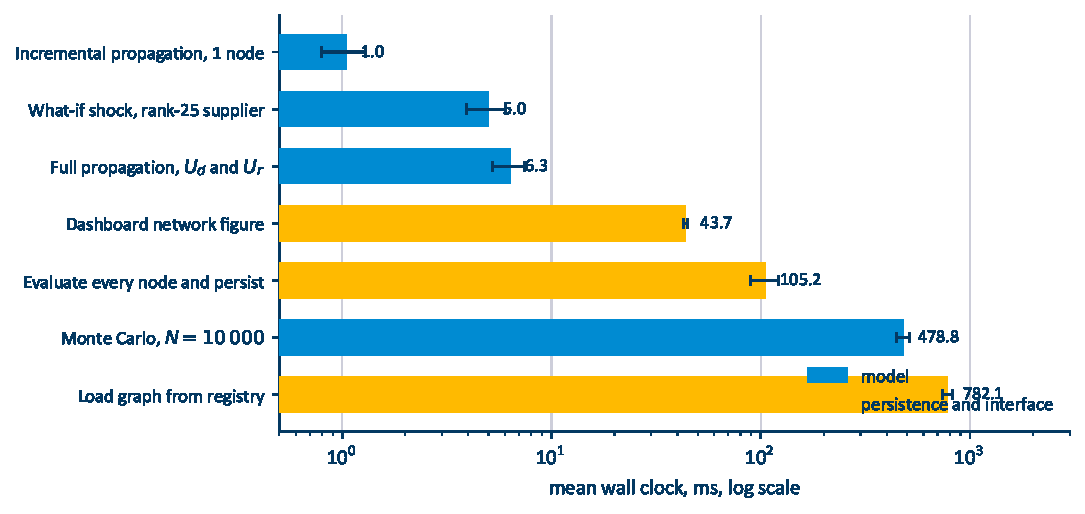
\includegraphics[width=0.92\linewidth]{Images/benchmarks.pdf}
    \caption[Measured performance at one thousand nodes]{The same seven operations on a log
    scale, model work in azure and persistence or interface work in ochre. Three orders of
    magnitude separate an incremental propagation from a graph load, and the operations a user
    waits on repeatedly are the fast ones.}
    \label{fig:benchmarks}
\end{figure}

Three readings matter. A full propagation of a thousand-node network costs $6.3$~ms, so the
recomputation triggered by a weekly review is imperceptible and the interactive what-if of
Section~\ref{sec:methods_impl} is genuinely interactive rather than nominally so. The
incremental pass is $6.1$ times faster than the full one, which is the empirical form of
Proposition~\ref{prop:propagation}(iii): the cone of a single changed node is a small
fraction of the graph, and everything outside it is read from cache without approximation.
And the Monte Carlo layer at $479$~ms is two orders of magnitude above the analytic path,
which is why it is an opt-in per project rather than the default, and why the memory guard
exists at all: at ten thousand draws over a thousand nodes the simulation holds
$10^{7}$ completion times in memory at once.

The one operation that dominates is loading the graph from the registry at $782$~ms, and it
is a persistence cost rather than a model cost. It is paid once per session, not per
recomputation, which is the reason it was left alone: optimising it would improve a number
nobody waits on twice.

%% ═══════════════════════════════════════════════════════════════════════════


%% ═══════════════════════════════════════════════════════════════════════════
\section{Observed Capacity: An Opening}
\label{app:opening}
%% ═══════════════════════════════════════════════════════════════════════════

Section~\ref{sec:limitations} records that the satellite work is reported as an
opening and claimed as no part of the contribution: nothing joins it to the
urgency model. It is set out here for that reason, with its protocol and data in
Appendix~\ref{app:volume}.

\label{sec:res_volume}
%% ═══════════════════════════════════════════════════════════════════════════

Every KPI reaching the six blocks arrives either through a manual weekly review or through a
scripted event, so a node's score is never fresher than its last submitted review, and the
capacity block in particular depends on the same operator whose declaration the adequacy
score exists to audit. The independence that Section~\ref{sec:res_discussion} identifies as
the precondition for the whole measurement is therefore not structurally guaranteed.

A second system, developed alongside the main work, addresses one part of that dependency by
estimating the physical capacity of a warehouse from public satellite imagery, which is an
observation no operator supplies and none can bias. It is an opening rather than a second
contribution: the two systems have not been connected, and no claim is made that they have.
The pipeline takes a coordinate, retrieves the building footprint from the French national
topographic database, retrieves 20~cm orthophotography and, where available, a LiDAR surface
model, and derives a storable volume as $0.80 \times \text{footprint} \times \text{height}$
and a transfer capacity as the equipped facade length divided by a dock pitch of $3.8$~m.
Both constants are calibrated rather than assumed, and Appendix~\ref{app:volume} gives each
with the sample behind it, together with the one that does not survive audit: the fill factor
of $0.80$ is attributed in the source to a 122-site calibration whose detailed output was not
retained, and recomputing it over the 68 sites still on disk gives a median of $0.97$. The
volumetric figures below carry that unquantified bias; the dock figures, which depend on the
pitch instead, do not.

\subsection{The Physical Limit and the Reframing}
\label{sec:res_volume_limit}

The original objective was to count loading docks. That objective is unreachable, and
establishing why is the most transferable result of this work.

An empty dock door under a canopy produces no measurable signal from directly overhead.
Measured contrast at verified empty bays is $0.18\sigma$, $0.22\sigma$ and $0.01\sigma$
across a full sweep of assumed depths, while occupied bays on the same facades register at
$5.3\sigma$ to $6.4\sigma$. The measurement is sensitive enough; the signal is absent.
Repeating the test on 8~cm very-high-resolution imagery leaves the doors equally invisible,
which shows the cause to be occlusion by the canopy roof rather than insufficient resolution.
A gain of $2.5\times$ in ground sample distance recovers no additional door: what improves
with resolution is everything except the quantity of interest. Any method claiming to count
empty doors one by one from a nadir view is recovering an artefact.

That finding splits the problem in two. Counting each door individually is not observable at
nadir, and no amount of resolution changes it. Recognising that a facade is equipped for
docking, and delimiting its extent, is observable, because the canopy, the apron and the bay
rhythm remain visible whether or not a vehicle is present. The second formulation is
learnable, and it is sufficient, because capacity is a function of equipped length rather
than of individually identified doors. Figure~\ref{fig:volume_proof} is the direct evidence:
three facades of 135~m, 105~m and 15~m on which the automatic trailer detector found no
vehicle at all, where individual doors are not resolvable and the bay markings and canopy
edge are.

\begin{figure}[htbp]
    \centering
    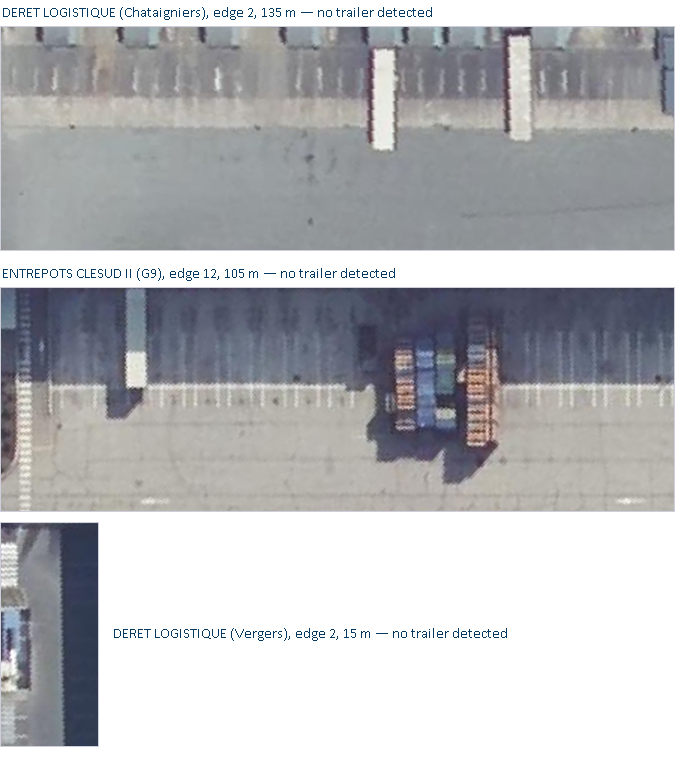
\includegraphics[width=0.72\linewidth, height=0.42\textheight, keepaspectratio]{Images/5.Volume/facade_proof_en.png}
    \caption{Equipped facades on which no trailer was detected}
    \label{fig:volume_proof}
\end{figure}

One reservation is recorded honestly. The proportion of sites showing no usable dock
signature was measured on a subsample that required vehicles to be present to establish
ground truth, and is therefore biased towards sites with vehicles. Five zero-shot approaches
were tried before the reframing and each was abandoned for a measured reason;
Appendix~\ref{app:volume} records them, because the reasons constrain what a successful
method can look like.

\subsection{Learned Dock-Zone Segmentation}
\label{sec:res_volume_seg}

The reframed problem was addressed by training a segmentation model to delimit equipped
facade zones directly. Table~\ref{tab:volume_training} gives the progression across four
training runs, read at the best epoch of each by mask mAP50-95.

\begin{table}[htbp]
\centering
\caption{Segmentation training progression}
\label{tab:volume_training}
\small
\begin{tabularx}{\linewidth}{l >{\centering\arraybackslash}X >{\centering\arraybackslash}X >{\centering\arraybackslash}X >{\centering\arraybackslash}X >{\centering\arraybackslash}X >{\centering\arraybackslash}X}
\toprule
\textbf{Run} & \textbf{Train / val} & \textbf{Image size} & \textbf{Precision} &
\textbf{Recall} & \textbf{mAP50} & \textbf{mAP50-95} \\
\midrule
1 & 86 & 640 & 0.461 & 0.404 & 0.363 & 0.155 \\
2 & 203 / 50 & 640 & 0.635 & 0.539 & 0.610 & 0.283 \\
3 & 351 / 91 & 640 & \textbf{0.702} & \textbf{0.606} & \textbf{0.618} & \textbf{0.305} \\
4 & 351 / 91 & 1280 & 0.652 & 0.547 & 0.570 & 0.272 \\
\bottomrule
\end{tabularx}
\end{table}

\begin{figure}[htbp]
    \centering
    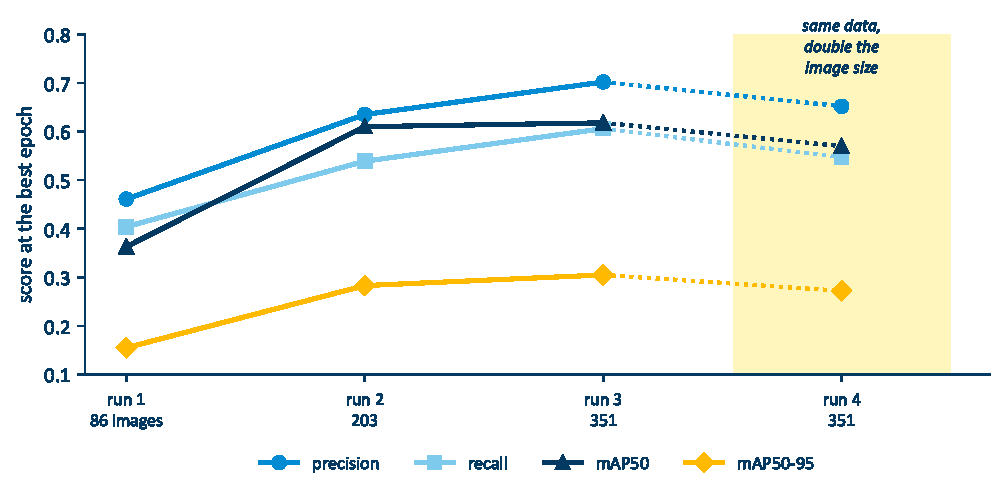
\includegraphics[width=0.94\linewidth]{Images/segmentation_runs.pdf}
    \caption[What moved the segmentation model]{The same four runs plotted. Runs~1 to~3 raise
    the training set at a fixed image size and every metric rises with it. Run~4 holds the set
    and doubles the image size instead, and every metric falls. The binding constraint was
    annotated data rather than resolution, which is a conclusion about the corpus and not
    about the architecture.}
    \label{fig:segmentation_runs}
\end{figure}

Figure~\ref{fig:segmentation_runs} makes the cause visible: quadrupling the training set from 86 to 351 images roughly
doubled mask mAP50-95. Resolution did not: run 4 is identical to run 3 except for a doubled
input size, and it is worse on every metric, so at a fixed data budget and a CPU-only
training budget the additional pixels cost more than they bought.

What is measured matters as much as the score. Standard detection metrics score shape
overlap, but the operational quantity is capacity, which depends only on the length of the
equipped zone: a polygon drawn too deep, or with imprecise edges, still yields the correct
dock count. The project therefore scores itself on the error in the derived dock count rather
than on mAP, and that business metric is the one used to decide whether a model is good
enough to deploy. On the reference run it reports a global bias of $-35\%$, a median error of
$62\%$ on images containing docks, and $89\%$ of true negatives correctly left empty, which
is a system that is directionally useful and quantitatively not yet trustworthy.

The pipeline runs end to end on a geographic area, retrieving footprints, presenting each to
the trained model, assigning predicted zones to the correct building and writing capacity
figures. One defect found during that deployment is recorded in Appendix~\ref{app:volume}
because it illustrates the difference between a model error and a systems error, as is the
annotation episode in which an automated third-party process reported 442 annotations as
verified and complete while having placed a zone along every edge of every building without
examining the imagery at all.

\subsection{What This Can and Cannot Feed}
\label{sec:res_volume_bridge}

The system supplies a storable volume, a pallet-position estimate and, where a dock zone is
detected, a transfer capacity and an occupancy ratio. Those map onto the capacity block of
Equation~\ref{eq:ur_local} and onto nothing else: it says nothing about lead time, cost or
emissions. Coverage is metropolitan France, bounded by the public data services it draws on.
The trained segmentation model is not yet wired into the production capacity path, which
still uses the zero-shot trailer method and its $36\%$ coverage. And the imagery is a
snapshot, so the resulting figure is a structural capacity rather than a live occupancy.

What it does change is the provenance of one input. A capacity figure derived from imagery is
not supplied by the operator whose declaration the adequacy score audits, which is precisely
the independence Section~\ref{sec:res_discussion} identifies as the precondition for the
measurement to mean anything. Figure~\ref{fig:volume_bridge} states where that input would
enter and, equally important, which blocks it would leave untouched.

\begin{figure}[htbp]
\centering
\begin{tikzpicture}[x=1cm, y=1cm, font=\scriptsize]

%% ── Bande haute : le systeme tel qu'il est livre ────────────────────────────
\node[titreBande, anchor=west] at (-0.9, 1.95) {As delivered};
\node[etiquette, anchor=west] at (1.75, 1.95) {the same observer supplies both sides};

\node[bloc, minimum width=2.0cm, minimum height=0.95cm] (opA) at (0.6, 0.55)
     {Operator\\[1pt]\textit{weekly review}};

\foreach \i/\lab in {0/{$u_{\text{time}}$}, 1/{$u_{\text{cap}}$}, 2/{$u_{\text{perf}}$},
                     3/{$u_{\text{risk}}$}, 4/{$u_{\text{cost}}$}, 5/{$u_{\text{co}_2}$}}
  \node[blocFort, minimum width=1.12cm, minimum height=0.62cm]
       (tA\i) at (3.55 + 1.22*\i, 1.15) {\lab};

\node[bloc, minimum width=1.9cm, minimum height=0.58cm] (ahpA) at (2.60, -0.45)
     {AHP $\rightarrow U_d$};

\node[blocFort, minimum width=1.35cm, minimum height=0.95cm] (adqA) at (11.9, 0.55)
     {$A(t)$};

\draw[fleche] (opA.east) -- (2.75, 0.55) -- (2.75, 1.15) -- (tA0.west);
\draw[fleche] (opA.south) |- (ahpA.west);
\draw[fleche] (tA5.east) -- (11.0, 1.15) -- (11.0, 0.82) -- (adqA.north west);
\draw[fleche] (ahpA.east) -- (11.0, -0.45) -- (11.0, 0.28) -- (adqA.south west);

\draw[fleche, dashed] (0.15, 1.03) .. controls (0.05, 1.72) and (1.15, 1.72) .. (1.05, 1.03);

\draw[altenGreyLine, line width=0.6pt] (-0.9, -1.15) -- (13.6, -1.15);

%% ── Bande basse : avec le canal observe ─────────────────────────────────────
\node[titreBande, anchor=west] at (-0.9, -1.45) {With observation};

\node[etiquette, anchor=west, text=altenOchreDark] at (3.05, -1.45)
     {broken for $u_{\text{cap}}$ alone};

\node[bloc, minimum width=2.0cm, minimum height=0.95cm] (opB) at (0.6, -2.75)
     {Operator\\[1pt]\textit{weekly review}};

\foreach \i/\lab in {0/{$u_{\text{time}}$}, 2/{$u_{\text{perf}}$}, 3/{$u_{\text{risk}}$},
                     4/{$u_{\text{cost}}$}, 5/{$u_{\text{co}_2}$}}
  \node[blocPale, minimum width=1.12cm, minimum height=0.62cm]
       (tB\i) at (3.55 + 1.22*\i, -2.15) {\lab};
\node[blocObs, minimum width=1.12cm, minimum height=0.62cm]
     (tB1) at (4.77, -2.15) {$u_{\text{cap}}$};

\node[bloc, minimum width=1.9cm, minimum height=0.58cm] (ahpB) at (2.60, -3.75)
     {AHP $\rightarrow U_d$};

\node[blocFort, minimum width=1.35cm, minimum height=0.95cm] (adqB) at (11.9, -2.75)
     {$A(t)$};

\draw[flechePale] (opB.east) -- (2.75, -2.75) -- (2.75, -2.15) -- (tB0.west);
\draw[fleche] (opB.south) |- (ahpB.west);
\draw[fleche] (tB5.east) -- (11.0, -2.15) -- (11.0, -2.48) -- (adqB.north west);
\draw[fleche] (ahpB.east) -- (11.0, -3.75) -- (11.0, -3.02) -- (adqB.south west);

%% la meme boucle qu'au-dessus, au meme endroit, mais rompue
\draw[flechePale, dashed] (0.15, -2.28) .. controls (0.05, -1.90) and (1.15, -1.90) ..
     (1.05, -2.28);
\draw[altenOchreDark, line width=1.1pt] (0.42, -2.10) -- (0.78, -1.74);
\draw[altenOchreDark, line width=1.1pt] (0.42, -1.74) -- (0.78, -2.10);

%% le canal observe, qui n'atteint qu'un bloc
\node[blocObs, minimum width=1.45cm, minimum height=0.55cm] (sat) at (1.05, -4.95)
     {satellite};
\node[blocObs, minimum width=1.55cm, minimum height=0.55cm] (bdt) at (3.30, -4.95)
     {footprint};
\node[blocObs, minimum width=1.75cm, minimum height=0.55cm] (ort) at (5.60, -4.95)
     {ortho 20\,cm};
\node[blocObs, minimum width=2.60cm, minimum height=0.55cm] (seg) at (8.55, -4.95)
     {dock-zone segmentation};
\node[bloc, minimum width=2.60cm, minimum height=0.95cm, draw=altenOchreDark,
      fill=white] (sorties) at (12.15, -4.95)
     {\texttt{volume\_m3}\\\texttt{palettes}\\\texttt{taux\_occupation}};

\draw[flecheObs] (sat) -- (bdt);
\draw[flecheObs] (bdt) -- (ort);
\draw[flecheObs] (ort) -- (seg);
\draw[flecheObs] (seg) -- (sorties);
\draw[flecheObs] (sorties.north) -- (12.15, -4.35) -- (4.77, -4.35) -- (tB1.south);

\end{tikzpicture}
\caption[Where observed capacity would enter the real-urgency model]{Where
satellite-observed capacity would enter the real-urgency model, and which blocks it does not
reach. Above, every block and the declaration itself originate with the same observer, which
is the circularity of Section~\ref{sec:res_discussion}. Below, one block of six is fed by an
observation no operator supplies, so the circular dependency is cut for that block; the other
five, greyed, still arrive through the weekly review.}
\label{fig:volume_bridge}
\end{figure}


\subsection{Reference tables}

The tables below define the terms of the model equations, list the campaign's network
and events, and record the two literature comparisons. Each is referred to from the
body at the point it applies.

\begin{table}[htbp]
\centering
\caption{DISCO technology stack}
\label{tab:disco_stack}
\begin{tabularx}{\linewidth}{lX}
\toprule
\textbf{Component} & \textbf{Technology / Value} \\
\midrule
Backend API    & Spring Boot + Java~21 \\
Database       & PostgreSQL (Azure) \\
Frontend       & Angular \\
Authentication & Player key / Azure AD SSO OAuth2 \\
Scores computed & CO\textsubscript{2}, Cost, Risk per supplier and itinerary, on $[1,10]$ \\
\bottomrule
\end{tabularx}
\end{table}

\begin{table}[htbp]
\centering
\caption[Aggregation and growth models found in the literature]{Aggregation and growth
models found in the literature. Figure~\ref{fig:aggregation_families} plots what each
one does.}
\label{tab:urgency_models}
\small
\begin{tabularx}{\linewidth}{>{\raggedright\arraybackslash}p{3.4cm} >{\raggedright\arraybackslash}p{3.6cm} >{\raggedright\arraybackslash}X}
\toprule
\textbf{Model} & \textbf{Formula} & \textbf{Where it appears} \\
\midrule
Linear in time & $U_0 + \lambda t$ & Deadline-sensitive scheduling
\autocite{cheng1996due} \\[3pt]
Hyperbolic in time & $K / (t_c - t)$, bounded & Temporal discounting
\autocite{steel2006integrating}; crash precursors \autocite{johansen2001finite} \\[3pt]
Weighted average of blocks & $\sum_m \omega_m u_m$ & Composite indicators
\autocite{greco2018} \\[3pt]
Noisy-OR over blocks & $1-\prod_m(1-u_m)^{\omega_m}$ & Combining independent causal evidence
\autocite{pearl1988probabilistic} \\
\bottomrule
\end{tabularx}
\end{table}

\begin{table}[htbp]
\centering
\caption{Temporal Motivational Theory parameters}
\label{tab:tmt_vars}
\begin{tabularx}{\linewidth}{llX}
\toprule
\textbf{Symbol} & \textbf{Concept} & \textbf{Operational role} \\
\midrule
$V(t)$ & Temporal motivational value & Dynamic task salience \\
$U$ & Objective utility & Task strategic importance \\
$E$ & Expectancy of success & Probability of task completion \\
$D(t)$ & Delay to deadline & Remaining safe execution window \\
$\Gamma$ & Impulsiveness parameter & Operator sensitivity to delay \\
$k$ & Sensitivity scaling parameter & Non-linear scaling of delay discounting \\
\bottomrule
\end{tabularx}
\end{table}

\begin{table}[htbp]
\centering
\caption[Precursors of delivery rupture]{The five families of precursor, and what each
contributes}
\label{tab:precursors}
\small
\begin{tabularx}{\linewidth}{@{}>{\raggedright\arraybackslash}p{2.5cm} X
                                 >{\raggedright\arraybackslash}p{3.3cm}@{}}
\toprule
\textbf{Family} & \textbf{Why it precedes rupture} & \textbf{Sources} \\
\midrule
Slack & The margin between a realistic lead time and the committed deadline. The only
indicator whose exhaustion is irreversible: a task with no slack left cannot be recovered
& \autocite{cohen2021assigning,bojarski2021,sun2020combating,sawik2013integrated} \\
\addlinespace
Capacity saturation & Adds waiting time a nominal lead time does not show, so a loaded system
carries a risk its announced schedule conceals
& \autocite{tomlin2006value,hosseini2019resilient,taghavi2024sustainable} \\
\addlinespace
Resource performance drift & Monitored through composite proxies, most often OEE, because
direct performance data is rarely available on the supplier side
& \autocite{mokhtar2019supplier,hlioui2017joint} \\
\addlinespace
Adverse-event exposure & Treated probabilistically, as failure probability times recovery
duration times impact severity
& \autocite{hosseini2020ripple,liu2021robust,hosseini2020bayesian} \\
\addlinespace
Cost signals & Symptoms of strain rather than causes: paying air freight to protect a deadline
is evidence the system is already compensating
& \autocite{heckmann2015critical,mokhtar2019supplier} \\
\bottomrule
\end{tabularx}
\end{table}

\begin{table}[htbp]
\centering
\caption[Multi-criteria methods compared]{The four methods on the three axes that matter for
a weekly-cadence instrument, with $n$ criteria and $q$ alternatives}
\label{tab:mcdm}
\small
\begin{tabularx}{\linewidth}{@{}>{\raggedright\arraybackslash}p{2.3cm} c
                                 >{\raggedright\arraybackslash}p{2.4cm} c X@{}}
\toprule
\textbf{Method} & \textbf{Judgements} & \textbf{Returns} & \textbf{Compens.} &
\textbf{Known weakness} \\
\midrule
AHP~\autocite{saaty1980analytic} & $n(n-1)/2$ & criterion weights, with a consistency ratio
& yes & rank reversal on adding an alternative; sensitive to cognitive noise during
elicitation~\autocite{dyer1990,triantaphyllou2024} \\
\addlinespace
BWM~\autocite{rezaei2015best} & $2n-3$ & criterion weights & yes & anchors on a best and a
worst the operator must be able to name \\
\addlinespace
Fuzzy BWM~\autocite{guo2017fuzzy} & $2n-3$ & fuzzy weights, defuzzified & yes & non-linear
programme; needs a feasible start, and consistency conditions were established only
later~\autocite{liang2020} \\
\addlinespace
PROMETHEE~II\newline \autocite{brans1986promethee} & $q(q-1)$ pairs per criterion
& a complete ranking of alternatives & \textbf{no} & not independent of irrelevant
alternatives: adding an alternative can invert two existing
ranks~\autocite{triantaphyllou2000multi} \\
\bottomrule
\end{tabularx}
\end{table}

\begin{table}[htbp]
\centering
\caption{Selection filter applied to each candidate block}
\label{tab:block_selection}
\small
\begin{tabularx}{\linewidth}{lX}
\toprule
\textbf{Criterion} & \textbf{Question asked of each candidate indicator} \\
\midrule
Causal link & Does the indicator have a plausible mechanism linking it to delivery
rupture? \\
\midrule
Observability & Can it be measured or credibly estimated from client, supplier or planning
data? \\
\midrule
Actionability & Can an operator act on it, or use it to decide? \\
\midrule
Non-redundancy & Does it add information not already carried by a retained indicator? \\
\bottomrule
\end{tabularx}
\end{table}

\begin{table}[htbp]
\centering
\caption{Terms of the propagation equations}
\label{tab:propagation_components}
\small
\begin{tabularx}{\linewidth}{llX}
\toprule
\textbf{Component} & \textbf{Type} & \textbf{Description} \\
\midrule
$U_{d,i}$, $U_{r,i}$ & Dependent variables & Propagated declared and real urgency at node
$i$ \\
$U_{d,\text{local},i}$, $U_{r,\text{local},i}$ & Input variables & Local urgency at node
$i$ after status-rule adjustment \\
$\gamma_{ik}$ & System parameter & Downstream demand attenuation coefficient on arc
$i \to k$ \\
$\beta_{ji}$ & System parameter & Upstream risk amplification coefficient on arc
$j \to i$ \\
$\text{Succ}(i)$, $\text{Pred}(i)$ & Structural sets & Nominal successors and predecessors
of node $i$ \\
\bottomrule
\end{tabularx}
\end{table}

\begin{table}[htbp]
\centering
\caption{Terms and parameters of the adequacy equations}
\label{tab:adequation_components}
\small
\begin{tabularx}{\linewidth}{llXl}
\toprule
\textbf{Component} & \textbf{Type} & \textbf{Description} & \textbf{Default} \\
\midrule
$F$ & Dependent variable & False urgency, from over-declaration & n/a \\
$H$ & Dependent variable & Hidden risk, from under-declaration & n/a \\
$\lambda_{\text{under}}$ & System parameter & Penalty weight on hidden risk & $2.25$ \\
$\lambda_{\text{over}}$ & System parameter & Penalty weight on false urgency & $1.0$ \\
$\alpha$ & System parameter & Psychophysical curvature & $0.88$ \\
$A$ & Dependent variable & Adequacy score, $100$ meaning perfect alignment & $[0,100]$ \\
\bottomrule
\end{tabularx}
\end{table}

\begin{table}[htbp]
\centering
\caption{The eight H\'ELIOS campaign nodes}
\label{tab:helios_network}
\small
\begin{tabularx}{\linewidth}{>{\raggedright\arraybackslash}p{3.1cm} >{\raggedright\arraybackslash}p{2.6cm} c X}
\toprule
\textbf{Node} & \textbf{Role} & \textbf{Rank} & \textbf{Real-world anchor} \\
\midrule
Orbitalys & Satellite prime, final customer & 0 & Fictional satellite programme,
contractual delivery pressure \\
AvioSys Int\'egration & Avionics integrator & 1 & Qualified-stock squeeze on avionics
tier-1 suppliers \\
\'Electis EMS & Electronics manufacturing services & 2 & EMS plants placed under
allocation, 2021 \\
CompoDis Europe & Component distributor & 3 & Distributor allocation and spot-market
premiums \\
TransGlobal Fret & Freight operator & 3 & Suez Canal blockage, West Coast port
congestion \\
NovaFab Semiconductors & Foundry, expected bottleneck & 4 & Composite of the Texas
winter-storm freeze and the Taiwan drought \\
Meridian Semi & Secondary foundry, inert backup arc & 4 & A foundry sold out through 2023,
the announced plan B that delivers nothing \\
SilPure Materials & Raw wafer supplier & 5 & Roughly 60\% of world wafer supply,
polysilicon price roughly tripling in 2021 \\
\bottomrule
\end{tabularx}
\end{table}

\begin{table}[htbp]
\centering
\caption{The twelve calibrated engine events}
\label{tab:helios_events}
\small
\begin{tabularx}{\linewidth}{c >{\raggedright\arraybackslash}p{2.3cm} >{\raggedright\arraybackslash}p{2.9cm} X}
\toprule
\textbf{Turn} & \textbf{Node} & \textbf{Event type} & \textbf{Real-world anchor} \\
\midrule
T3 & NovaFab & Demand spike & Automotive reorders on sold-out slots, Nov.\ 2020 \\
T5 & CompoDis & Supplier delay & Distributor moves to allocation, Jan.\ 2021 \\
T6 & NovaFab & Accident (critical) & Texas winter-storm fab freeze, Feb.\ 2021 \\
T7 & NovaFab & Demand spike & Reorders after a competitor's fab fire, Mar.\ 2021 \\
T7 & TransGlobal & Transport disruption & Suez Canal blockage, six days, Mar.\ 2021 \\
T10 & NovaFab & Material shortage & Taiwan drought, ultrapure-water rationing, Jun.\ 2021 \\
T12 & \'Electis & Capacity loss & Southeast-Asia backend lockdowns, Aug.\ 2021 \\
T12 & TransGlobal & Transport disruption & Shift to saturated air freight, Aug.\ 2021 \\
T13 & CompoDis & Demand spike & Bullwhip over-ordering, Sep.\ 2021 \\
T14 & TransGlobal & Transport disruption & West Coast port congestion, Oct.\ 2021 \\
T14 & CompoDis & Tariff increase & Allocation spot premiums, Oct.\ 2021 \\
T16 & SilPure & Tariff increase & Polysilicon price pass-through, Dec.\ 2021 \\
\bottomrule
\end{tabularx}
\end{table}

\begin{table}[htbp]
\centering
\caption{Final per-node snapshot of the arm A project}
\label{tab:armA_snapshot}
\small
\begin{tabularx}{\linewidth}{l >{\centering\arraybackslash}X >{\centering\arraybackslash}X >{\centering\arraybackslash}X >{\centering\arraybackslash}X >{\centering\arraybackslash}X}
\toprule
\textbf{Node} & $U_d$ & $U_r$ & $A$ & $F$ & $H$ \\
\midrule
Orbitalys & 0.409 & 1.000 & 15.3 & 0.000 & 0.591 \\
AvioSys Int\'egration & 0.727 & 0.698 & 95.2 & 0.029 & 0.000 \\
\'Electis EMS & 0.914 & 0.965 & 82.9 & 0.000 & 0.052 \\
CompoDis Europe & 0.882 & 1.000 & 67.5 & 0.000 & 0.118 \\
TransGlobal Fret & 0.819 & 1.000 & 56.0 & 0.000 & 0.181 \\
Meridian Semi & 0.841 & 0.998 & 60.1 & 0.000 & 0.157 \\
NovaFab Semiconductors & 0.912 & 0.915 & 98.5 & 0.000 & 0.003 \\
SilPure Materials & 0.876 & 0.304 & 48.9 & 0.572 & 0.000 \\
\bottomrule
\end{tabularx}
\end{table}

\begin{table}[htbp]
\centering
\caption{The time block at turn 6}
\label{tab:u_time_turn6}
\small
\begin{tabularx}{\linewidth}{lX}
\toprule
\textbf{Node} & \textbf{$u_{\text{time}}$} \\
\midrule
Orbitalys & $7.3 \times 10^{-9}$ \\
AvioSys Int\'egration & $1.2 \times 10^{-8}$ \\
\'Electis EMS & $0.0$ \\
CompoDis Europe & $0.99996$ \\
TransGlobal Fret & $1.7 \times 10^{-4}$ \\
Meridian Semi & $2.9 \times 10^{-9}$ \\
NovaFab Semiconductors & $0.0216$ \\
SilPure Materials & $0.0$ \\
\bottomrule
\end{tabularx}
\end{table}


\subsection{Summary tables of the conclusion}

The three tables below summarise, in one place, what each research question returned,
what each contribution rests on, and what each item of future work takes. Each is
referred to from Section~\ref{sec:Conclusion}.

\begin{table}[htbp]
\centering
\caption{What each research question returned}
\label{tab:rq_answers}
\small
\begin{tabularx}{\linewidth}{>{\raggedright\arraybackslash}p{2.0cm} X}
\toprule
\textbf{Question} & \textbf{Answer} \\
\midrule
RQ1 \newline multi-block real urgency & Specified, implemented and exercised over two chains.
The construction works and is exactly decomposable, which is what allowed its own defect to
be found: five blocks behaved as intended and the time block was structurally unable to
respond to a disruption, because the event engine wrote to no quantity it reads. That path
has since been built and measured (Section~\ref{sec:res_repair}). The aggregation is only as
informative as its inputs, and the campaign that produced the negative result ran with three
of the six blocks inert. \\[3pt]
\midrule
RQ2 \newline adequacy formulation & Bounded, interpretable and reconstructible term by term.
Its validity splits by granularity. At node level it discriminates and does so early:
Section~\ref{sec:res_targeting} reports six consecutive turns on which the flagged set is a
subset of the eventually failing set, with no false alarm, ahead of any public sign of the
crisis. At the granularity of a probability attached to a node-week it was not demonstrated,
and Section~\ref{sec:res_mechanism} attributes that to one repairable cause rather than to the
formulation. Usable today for triage, not yet for probability. \\[3pt]
\midrule
RQ3 \newline prioritisation and criticality & AHP and Fuzzy BWM elicitation, PROMETHEE~II
outranking and systematic shock simulation combine into a working ranking that placed the
expected bottleneck at the top. Two behaviours bound it. The criticality index degenerated
when many nodes saturated at once, which a log-survival sort key has since addressed
(Section~\ref{sec:res_repair}); the outranking inherited a perfect correlation between two of
its criteria, which the tool flagged on its own. \\[3pt]
\midrule
RQ4 \newline validation, and the effect of display & Operationalised as a persistent twin and
exercised through two pre-registered campaigns. Five of six hypotheses are not confirmed and
H5 on urgency contagion is confirmed. On the second half of the question the answer is
unambiguous within its population: at first exposure no declarant on either chain revised
upward, and across all exposed turns of the second chain upward revisions outnumber downward
ones $26$ to $9$. The display transfers authority to the model rather than sedating the
operator. \\
\bottomrule
\end{tabularx}
\end{table}

\begin{table}[htbp]
\centering
\caption[The five contributions, measured and bounded]{Each contribution, the measurement
behind it, and what bounds it}
\label{tab:contributions}
\footnotesize
\begin{tabularx}{\linewidth}{@{}l >{\raggedright\arraybackslash}p{4.6cm} X@{}}
\toprule
& \textbf{Measurement} & \textbf{Bound} \\
\midrule
\textbf{C1} & 3 nodes flagged over the 6 turns before the crisis is public; 3 of 3 later miss
an \emph{originally committed} deadline; 0 false alarms; worst case flagged 8 turns ahead; one
flag on a node declaring $U_d = 0.001$
& 4 positives, Wilson $[0.44, 1.00]$; signal weakens once the crisis is public, so the scope
is early warning \\
\addlinespace
\textbf{C2} & noisy-OR real urgency, bidirectional DAG propagation, consistency-gated
declaration, asymmetric penalty: specified, implemented, operable, exactly decomposable
& fills the combination Section~\ref{sec:lit_gaps} finds absent; a claim about the reviewed
literature, not about optimality \\
\addlinespace
\textbf{C3} & Brier skill $-3.4$ to $-6.9$; 21 confident forecasts, 0 materialised. Cause: the
accumulated-delay field written non-zero \emph{exactly zero times}; block numerically zero at
6 of 8 nodes mid-crisis
& a count, so sample size does not bear on it; after repair $-0.553 \to -0.216$ at 4 weeks,
badly wrong to less wrong \\
\addlinespace
\textbf{C4} & 8 of 8 declarants revised down or were confirmed, 0 up, on first exposure, 2
turns before the critical event; both arms carry numerically identical forecasts
& attributable to the display, for a population of agents; human extension unestablished
(Assumption~\ref{as:sincerity}) \\
\addlinespace
\textbf{C5} & naive target: base rate $5.0\% \to 38.7\%$, apparent skill $\times 5$,
discrimination unchanged. Original-commitment target: AUC $0.485 \to 0.654$, skill
$-3.36 \to -0.55$
& the three targets disagree by more than any modelling decision in this work; no figure is
quotable without its definition \\
\bottomrule
\end{tabularx}
\end{table}

\begin{table}[htbp]
\centering
\caption[The eight items of future work]{Each item, what it costs, and what it unblocks}
\label{tab:futurework}
\footnotesize
\begin{tabularx}{\linewidth}{@{}p{0.4cm} >{\raggedright\arraybackslash}p{3.5cm} X
                                 >{\raggedright\arraybackslash}p{2.0cm}@{}}
\toprule
& \textbf{Item} & \textbf{What it takes} & \textbf{Cost} \\
\midrule
\multicolumn{4}{@{}l}{\textbf{\color{altenOchreDark}Before the framework can be evaluated
fairly}} \\
\addlinespace
F1 & Separate misperception from discretion
& Instrument the escalation channel, so the interval between recognising and communicating
becomes observable; or read the free-text notes the system already collects, in which second
chain declarants stated an intent to delay contacting customers while marking near-maximal
severity in the same submission
& none for the second route \\
\addlinespace
F2 & Widen the evidence base
& More chains, longer horizons, more milestones. Three routes without new science: replay
documented disruptions on the same harness; instrument a live chain through the weekly review,
already supported; generate synthetic scale for the calibration layer, keeping the real
campaigns as the evaluation set
& scenario authoring \\
\addlinespace
F3 & Run the human campaign, outcome definition pre-registered
& Protocol, hashed data pack and scripts are ready. Run against the \emph{repaired} model.
Arm~C in its agent version met 5 milestones of 11 on original commitment against 5 of 11 for
arm~A: it changed \emph{which} milestone was met, saving one and replanning one that would
have held. That is the quantity to power for
& eight participants,\newline nine days \\
\addlinespace
\multicolumn{4}{@{}l}{\textbf{\color{altenAzureDark}And then}} \\
\addlinespace
F4 & Fill the indicators, rebuild the calibration label on the product's target
& Coverage rose $25.6\% \to 49.1\%$ on completion from public figures, activating all six
blocks and exposing a model bug undetectable on an empty database. The post-hoc calibrator
labels an event at exactly $t+1$ where the product reads a miss over $(t, t+4]$, which costs
$0.721 \to 0.580$ of four-week AUC. Blocked on the synthetic factory recording milestone truth
& concrete, blocked \\
\addlinespace
F5 & Smooth the milestone alarm
& It moves from $0.05$ to $1.00$ in a single turn: correct, and unusable as advance warning
& low \\
\addlinespace
F6 & Make the forecast state its own ignorance, and control the display
& Make the horizon salient so a low four-week figure cannot read as general safety; state the
risk classes not covered. Arm~B is not blinded, and turns carrying a deliberately
uninformative forecast would separate the effect of the content from the effect of being
given a number at all
& low \\
\addlinespace
F7 & Connect the observed capacity channel
& Wire the trained segmentation into the production capacity path in place of the
trailer-span method; re-measure the no-signature rate on an unbiased draw; recollect the
regulatory corpus to re-derive the fill factor. The LiDAR surface model is the most promising
unexplored route, the canopy step sitting several metres below the main roof, which would
correct the $0$ to $14.4$~m overhang now displacing the apron boundary
& medium \\
\addlinespace
F8 & Broaden elicitation, couple the platforms
& Multi-expert AHP aggregating several judgements per node; couple SupplyScore with the DISCO
platform it runs alongside. Both depend on what a repaired system shows
& medium \\
\bottomrule
\end{tabularx}
\end{table}
